\documentclass[a4paper,10pt]{report}
\usepackage[utf8x]{inputenc}
\usepackage[T1]{fontenc}
\usepackage[french]{babel} 
\usepackage{lmodern}
\usepackage{makeidx}
\usepackage{graphicx}
\usepackage{verbatim}
\usepackage{moreverb}
\usepackage{listings}
\usepackage{color}

\lstset
{
escapeinside={(*}{*)},
language=C,
basicstyle=\footnotesize,
numbers=left,
numberstyle=\normalsize,
numbersep=7pt,
captionpos=b
}

\title{Rapport de développement de l'application SolidSnake}
\author{Lisa Aubry Alban Chazot Korlan Colas Anthony Gourd}
\date{\today}

\pdfinfo{
  /Title    (Rapport de d\'eveloppement pour l'application SolidSnake)
  /Author   (Lisa Aubry, Alban Chazot, Korlan Colas, Anthony Gourd)
  /Creator  (Lisa Aubry, Alban Chazot, Korlan Colas, Anthony Gourd)
  /Producer (Lisa Aubry, Alban Chazot, Korlan Colas, Anthony Gourd)
  /Subject  (Application ``SolidSnake''; résolution du algorithmique du casse-tête ``Snake Cube'')
  /Keywords ()
}

\makeindex
\begin{document}

\begin{titlepage}
  \begin{center}

    % Upper part of the page. The '~' is needed because \\
    % only works if a paragraph has started.
    
\includegraphics[scale=1]{img/insacvl.jpg}~\\[1.5cm]

    \textsc{\LARGE INSA - CVL}\\[2cm]

    \textsc{\Large Rapport de développement}\\[1.5cm]

    % Title
    { \huge \bfseries Projet application\\[0.4cm] }
    \today
    
    \vfill

    % Author and supervisor
    Auteurs :\textsc{Aubry} Lisa, \textsc{Chazot} Alban, \textsc{Colas} Korlan, \textsc{Gourd} Anthony - Promotion 2017\\
    \emph{Tuteur :} P.\textsc{Clemente}\\
  \end{center}
\end{titlepage}

\begin{abstract}
Compte rendu portant sur le projet application effectué lors de la première année de formation à la Sécurité et aux Technologie de l'Informatique (STI) à l'INSA Centre Val de Loire
\end{abstract}

\tableofcontents

\chapter*{Introduction}
Véritables défis pour leurs utilisateurs, les casse-tête sont des objets de divertissement axés sur la réflexion, la logique ou les mathématiques. Ces jeux individuels se déclinent en plusieurs catégories, observant divers degrés de complexité et étant plus ou moins ludiques. Parmi ces grandes familles, on trouve celle des casse-tête mécaniques dont les origines remontent jusqu’à l’un des plus grands mathématiciens de l’antiquité, Archimède. Fort de son goût pour les énigmes, il s’est employé à transposer les pratiques mathématiques à des problèmes récréatifs, donnant entre-autre naissance au Syntémachion, le premier des casse-tête géométrico-mécanique. Puis l’histoire de ces casse-tête a jalonné les siècles et le monde, pour enfin connaître un développement accru à la fin du XVIIIe siècle. En Occident, ce développement a notamment été encouragé par la publication de Puzzles old and new par le Prof. Hoffmann et, encore une fois, pour sa résonance particulière dans le milieu des mathématiques. Les XIXe et XXe siècles seront marqués respectivement par l’invention des désormais célèbres Tangram (Chine) et Rubik’s Cube (Hongrie).\newline

À la lumière des algorithmes et des programmes informatiques, ces casse-tête prennent une autre dimension. Ils ouvrent la porte à de nouveaux enjeux, de nouveaux défis. C’est ainsi que l’on dénombra 536 solutions au casse-tête inventé par Archimède et que l’on explora les solutions émanant des 4,3.10\up{19}  positions de départ du Rubik’s Cube. De la fasciation suscitée par ces casse-tête est née une multitude d’algorithmes puis d’applications capables de les résoudre et d’en calculer toutes les solutions. Ces travaux ont été rendus possibles par l’avancée des technologies informatiques, le déploiement des architectures multi-cœurs et du calcul partagé.\newline

C’est dans cette optique que nous nous sommes attelés à développer une application autour d’un casse-tête mécanique plutôt méconnu, le Snake Cube. Cette méconnaissance a sans doute favorisé une vision authentique du problème, nous avons apprivoisé le Snake Cube et nous en avons compris les rouages au fur et à mesure que l’analyse préliminaire s’étayait sur le papier. Grâce à la combinaison de préceptes algorithmiques et mathématiques, nous avons déterminé le schéma de résolution du casse-tête. Ensuite l’application s’est prolongée avec le développement d’une interface homme-machine fluide et l’implémentation du jeu de l’utilisateur, lui permettant de manier lui-même un Snake Cube virtuel. À la fin de ce projet, il était nécessaire de fournir des résultats fidèles et complets quant aux solutions proposées et ce dans des temps de calculs acceptables. Mais outre ces impératifs de résultats, nous avons gardé à l’esprit que cette application devait être jouable et réellement utilisable. Il nous paraissait important qu’une fois fini, ce projet pouvait et devait en intéresser d‘autres que nous. Puisque finalement, qui n’a jamais capitulé devant un casse-tête ou une énigme difficile à résoudre ? À ceux-là et aux autres, férus de casse-tête mécaniques ou d’algorithmes, nous leur proposons une solution au Snake Cube, et bien plus encore.


\part{Analyse du sujet}
Le Snake Cube (ou cube serpent en français) est un casse-tête géométrique à trois dimensions appartenant à la famille des casse-tête mécaniques. Cette famille, dont fait parti le Rubik’s Cube, recouvre l’ensemble des jeux de réflexion basés sur la manipulation d’un objet tridimensionnel, afin de lui donner un agencement précis.


\begin{figure}[h]
 \centering
 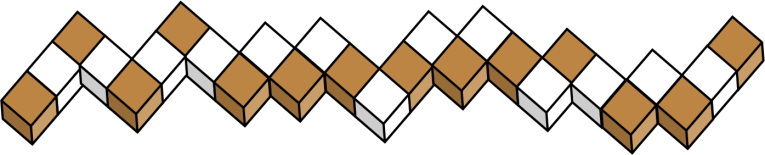
\includegraphics[scale=0.5,keepaspectratio=true]{img/snakeCubeFlat.png}
 \caption{Snake Cube déplié}
 \label{snakeFlat}
\end{figure}

Ce casse-tête se présente généralement comme une succession de 27 petits cubes en bois, reliés les uns aux autres par un fil élastique qui les traverse de part en part. Lorsque tous les cubes sont mis sur le même plan, la forme du puzzle s’apparente à un serpent  (Figure~\ref{snakeFlat}). Pour résoudre le puzzle, il faut manier le serpent afin de le ramener à une forme entièrement cubique telle que présentée ci-dessous (Figure~\ref{snakeSolved}). Dans la suite de cette partie et pour éviter les ambiguïtés, les petits cubes qui forment le serpent seront appelés \textbf{unités} tandis que le mot cube désignera plutôt le volume final visible sur la figure~\ref{snakeSolved}.

\begin{figure}[h]
 \centering
 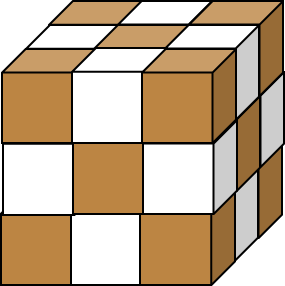
\includegraphics[scale=0.5,keepaspectratio=true]{img/snakeCubeSolved.png}
 \caption{Snake Cube résolu}
 \label{snakeSolved}
\end{figure}

\newpage Comme mentionné précédemment, les unités sont reliées entre elles ce qui les rend totalement indissociables. Ainsi, les manipulations pouvant être effectuées sur le puzzle sont réduites à des rotations. La Figure~\ref{snakeMove} illustre une manipulation réalisée sur le serpent présenté figure~\ref{snakeFlat}. De plus, on remarque que les rotations conduisant à modifier la forme de la figure s’effectuent toujours au niveau des coins du serpent. Cette particularité sera notamment exploitée lorsque l’on traitera de la résolution du casse-tête.

\begin{figure}[h]
 \centering
 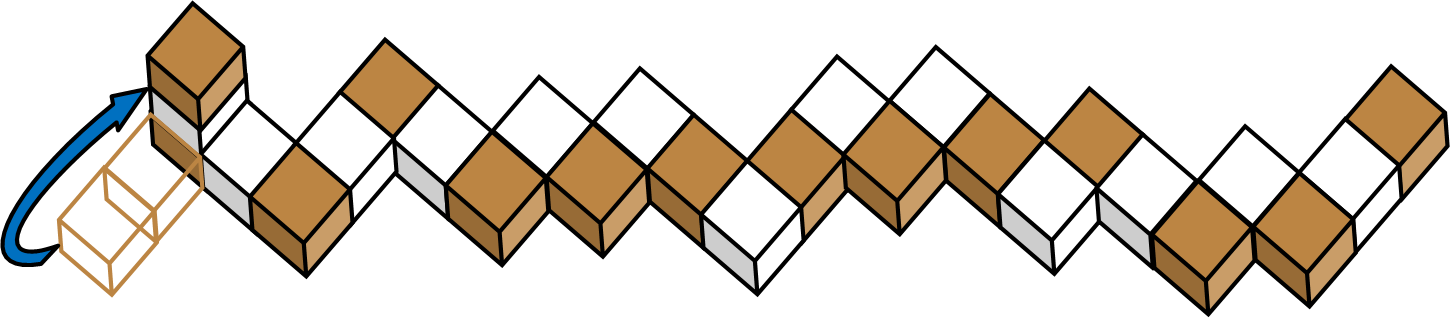
\includegraphics[scale=0.3,keepaspectratio=true]{img/snakeCubeMove.png}
 \caption{Exemple de manipulation du Snake Cube}
 \label{snakeMove}
\end{figure}

Notons également  que pour une figure finale donnée (ici une cube 3x3x3), il existe une multitude de formes de serpents correspondantes. Les serpents les plus connus sont disponibles dans l'application. De manière moins classique, on trouve aussi dans le commerce des serpents permettant de réaliser des cubes 4x4x4. À notre connaissance il n’existe pas de casse-tête correspondant à des Snake Cubes de tailles supérieures.

\chapter{Description des objectifs} 
Dans un premier temps, notre objectif consiste en l’implémentation d’une application capable de résoudre des Snake Cubes. L’utilisateur fournit au résolveur deux paramètres essentiels : la définition d’un serpent initial ainsi qu’un volume final. Ensuite l’application automatise la tâche de recherche pour présenter à l’utilisateur la liste de solutions correspondant au problème. Les solutions devront être présentées de manières claires avec, pour chacune d’entre elles, la possibilité pour l’utilisateur de la visionner pas-à-pas ou bien encore de revenir en arrière. Une première contrainte évidente liée à cet objectif concerne le temps nécessaire au calcul. Ainsi, il va de soi que le résolveur devra à la fois s’employer à utiliser des méthodes de calcul pertinentes et être capable de ne pas rechercher des solutions redondantes. Cette redondance traduit en fait le caractère symétrique de plusieurs solutions. 

Dans un second temps, nous proposons à l’utilisateur un mode interactif où celui-ci pourra tenter de résoudre virtuellement le casse-tête. En termes de contraintes, ce versant de l’application nécessite très peu de calcul. Néanmoins, il exige une réflexion accrue concernant la représentation graphique. En effet, il faut ici proposer au joueur un environnement en 3 dimensions à la fois clair et maniable ainsi qu’un panel de fonctionnalités rendant l’application intuitive. 

\part{Résolution du casse-tête}
Dans cette partie nous allons exposer les principes algorithmiques qui sous-tendent le fonctionnement du résolveur. Cette approche, bien que dénuée de détails techniques et autres soucis d’implémentation, proposera une réponse à nos différents objectifs tout en tenant compte de certaines des contraintes citées précédemment.  Nous nous baserons ici sur la résolution d’un cube 3x3x3 à l’aide du serpent présenté précédemment, le Cubra Orange. 
\chapter{Principe de la résolution}
\section{Quelques définitions}

Tout d’abord, deux éléments constituent la base de l’algorithme de résolution :\newline

\begin{itemize}
 \item le serpent, ici le Cubra Orange, composé de 27 unités reliées entre elles
 \item le volume final, ici un cube 3x3x3
\end{itemize}

\vspace{0.5cm}

Le volume final est définit par ses coordonnées, fixées, dans l’espace. Le serpent est quant à lui définit par sa forme qui découle de la nature de chacune des unités qui le composent. En effet, il faut distinguer trois types d’unité du serpent (Figure~\ref{snakeUnits}) :\newline

\begin{itemize}
 \item \textcolor{red}{les extrémités}
 \item \textcolor{blue}{les unités droites}
 \item \textcolor{green}{les coins}
\end{itemize}

\begin{figure}[h]
 \centering
 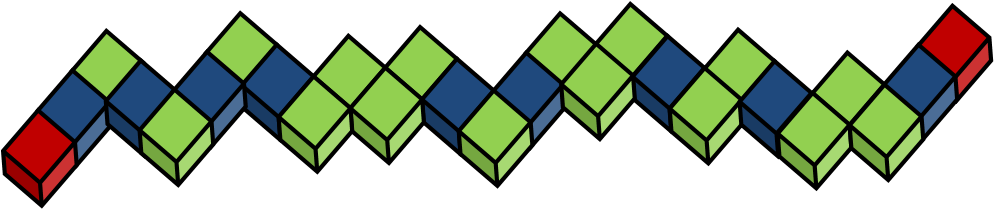
\includegraphics[scale=0.5,keepaspectratio=true]{img/unitTypes.png}
 \caption{Natures des unités du Cubra Orange}
 \label{snakeUnits}
\end{figure}

\clearpage
\section{Construction d’un arbre n-aire}
La résolution s’effectue de manière linéaire, en considérant tour à tour chacune des unités du serpent. Le principe est de placer temporairement l’unité considérée à l’intérieur du volume final en fonction de l’emplacement et de la nature de l’unité précédente. On construit ainsi une branche d’un arbre n-aire qui est le cœur de l’algorithme de résolution. Chaque nœud correspond à une unité associée à un couple coordonnées-direction.

Ici il est important de comprendre que ce travail s’effectue de telle sorte que chaque nouvelle unité soit nécessairement placée à l’intérieur du volume final. En tenant compte de cette contrainte et en fonction des emplacements choisis précédemment, on peut constater deux comportements pour une branche donnée. 

Soit on arrive à une impasse, c’est-à-dire qu’une configuration donnée ne permet pas de placer l’unité suivante sans sortir du volume ou la placer sur une autre unité. Dans ce cas, la branche avorte, il faut alors remonter dans l’arborescence jusqu’au prochain nœud qui a donné plusieurs fils. Ce cas de figure est illustré sur les figures~\ref{pathAbort} et~\ref{pathAfter}. Les flèches horizontales représentent les liens de fraternité dans l’arborescence et les flèches verticales représentent les liens de paternité. Ici on a construit six vecteurs initiaux, c’est-à-dire les couples coordonnées-direction possibles pour la première unité. Puis le premier nœud est devenu le nœud courant et a lui-même engendré des fils, en fonction des vecteurs possibles pour la deuxième unité. Et ainsi de suite jusqu’à ce que le nœud représenté en rouge devienne le nœud courant. À ce stade, on admet que ce nœud ne puisse pas engendrer de fils pour une des raisons évoquées précédemment. Cette branche va donc avorter. On va supprimer le nœud rouge et remonter jusqu’à son père (en vert). Si celui-ci a un frère, comme c’est le cas ici avec le nœud bleu, c’est ce frère qui devient le nouveau nœud courant. Il convient de supprimer également le nœud vert qui a généré le sous arbre menant à une impasse.  Ensuite la résolution peut suivre son court, et le nœud bleu générera à son tour ses fils (figure~\ref{pathAfter}).

\begin{figure}[h]
 \centering
 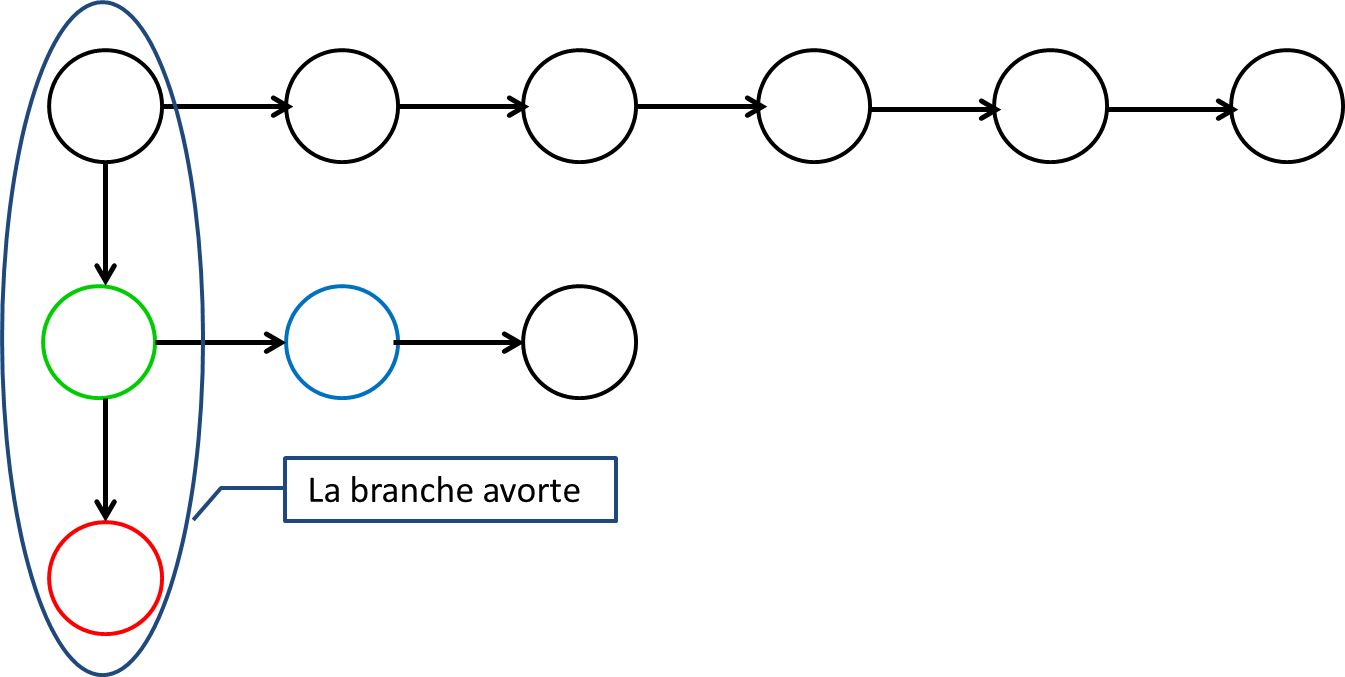
\includegraphics[scale=0.3,keepaspectratio=true]{img/pathAbort.png}
 \caption{Exemple d'une branche qui avorte}
 \label{pathAbort}
\end{figure}

\newpage

\begin{figure}[h]
 \centering
 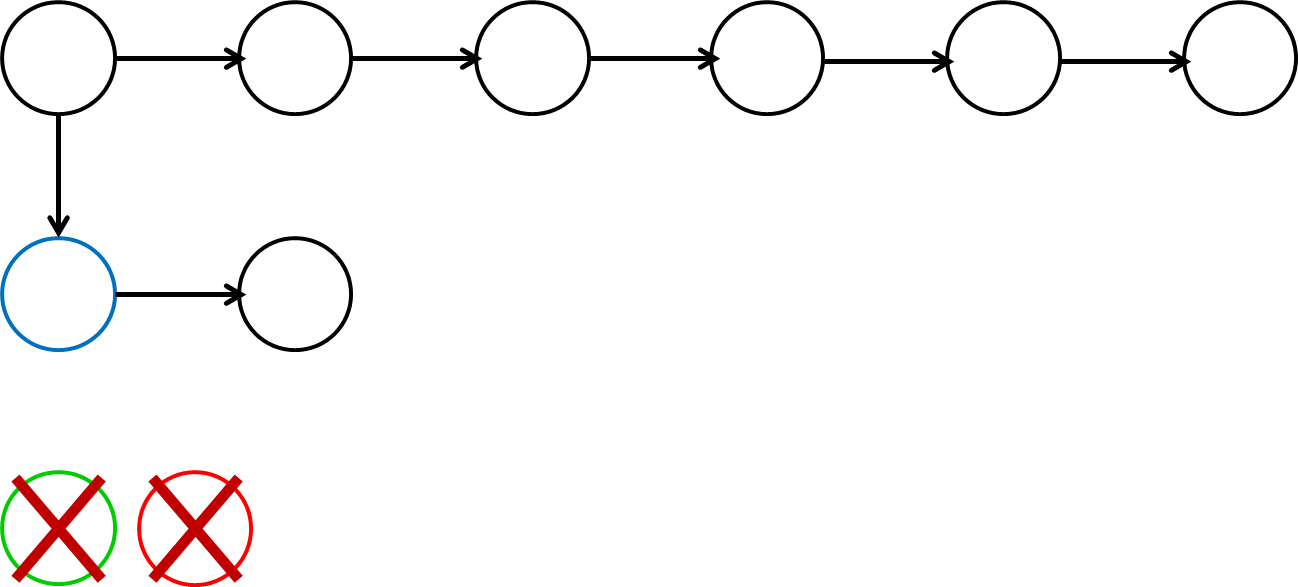
\includegraphics[scale=0.3,keepaspectratio=true]{img/pathAfter.png}
 \caption{Arbre après modifications}
 \label{pathAfter}
\end{figure}

Le deuxième cas de figure est celui où l’on réussit à placer toutes les unités du serpent à l’intérieur du volume. Dans ce cas, la branche aboutit et la succession de ses nœuds depuis la racine constitue une solution au problème. Il faut alors garder cette solution en mémoire puis, comme dans le cas précédent, remonter dans l’arborescence pour chercher des solutions supplémentaires. 

\section{Méthode de calcul des couples coordonnées-direction des nœuds fils}
Lorsqu’un nœud devient le nœud courant, il convient que ses fils soient générés dans l’arbre. Cela consiste notamment à leur attribuer un couple coordonnées-direction dans l’espace. Ce qu’il faut voir ici, c’est que le résultat de cette opération découle de la nature du nœud fils et du couple coordonnées-direction du père. Dans la suite de cette partie, on se placera dans un repère orthonormé (O ; x, y, z). 
Pour calculer les coordonnées des fils d’un nœud, il suffit d’ajouter ses coordonnées avec sa direction. La figure suivante illustre ce procédé. Le nœud marron est le nœud courant et le nœud blanc est son fils. Les coordonnées du fils découlent de la position du père ainsi que de sa direction, matérialisée par la flèche marron. On constate alors que, pour un nœud père donné, tous les fils qu’il va engendrer auront le même triplet de coordonnées dans l’espace. 

\begin{figure}[h]
 \centering
 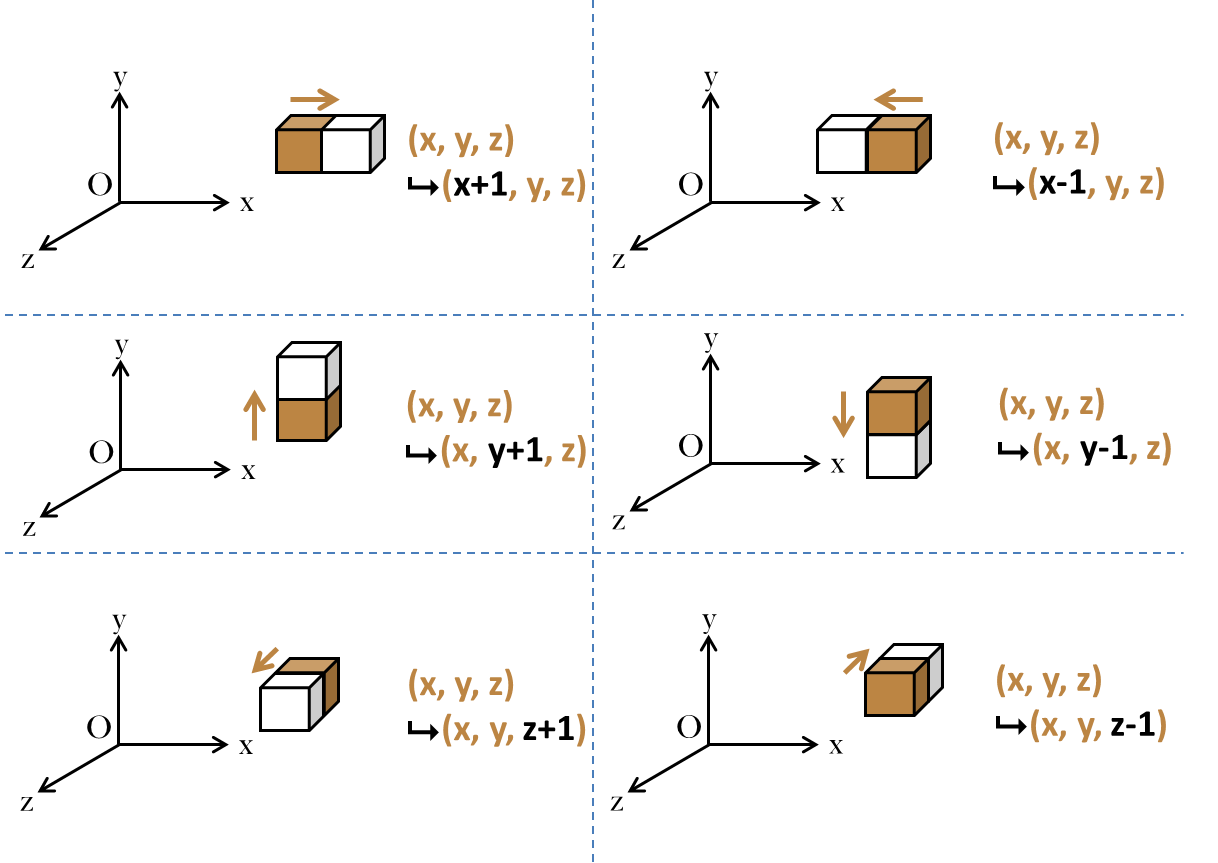
\includegraphics[scale=0.5,keepaspectratio=true]{img/buildChildren.png}
 \caption{Calcul des coordonnées des fils pour six pères différents}
 \label{buildChildren}
\end{figure}

La différence entre les fils d’un nœud intervient lors du calcul de leur direction. Deux cas de figure sont alors à envisager :
\begin{itemize}
 \item le nœud fils correspond à une unité droite (voir figure 4), dans ce cas, un seul nœud fils sera créé et celui-ci héritera de la direction de son père
 \item le nœud fils correspond à un coin, dans ce cas, plusieurs nœuds fils seront créés avec des directions différentes de celle du père
\end{itemize}
 
La figure~\ref{buildCornerChildren} illustre le fonctionnement de l’arbre pour placer la 3e unité du serpent à partir d’un nœud donné. Les flèches indiquent les directions associées au dernier cube placé. À la hauteur n, on a déjà positionné les deux premières unités et la 2e unité a pour direction droite.  Étant donné que la 3e unité est un coin (voir figure 4), il convient que la direction change entre la 2e et la 3e unité. Ainsi, les directions possibles pour la 3e unité sont : bas, derrière, devant et haut, d’où les quatre nœuds représentés à la hauteur n+1. 
NB : on peut d’ores et déjà remarquer que les directions devant et haut vont déboucher sur une configuration interdite car la prochaine unité créée sortira du cube.

\begin{figure}[h]
 \centering
 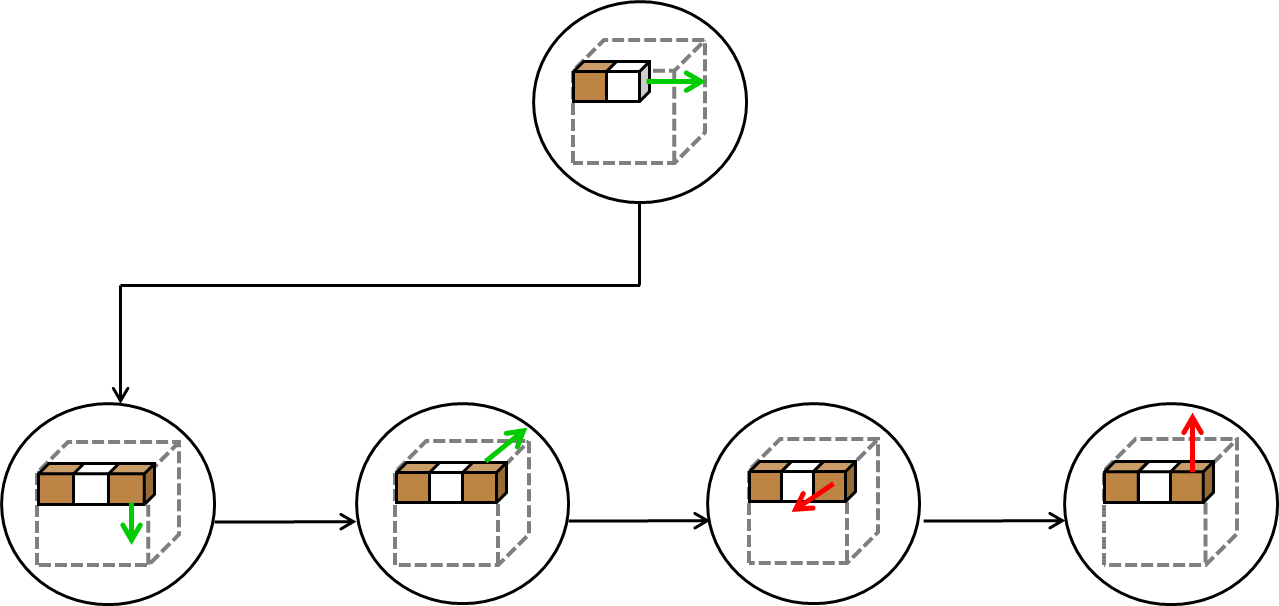
\includegraphics[scale=0.5,keepaspectratio=true]{img/buildCornerChildren.png}
 \caption{Exemple de création des fils pour un coin}
 \label{buildCornerChildren}
\end{figure}

\clearpage
\section{Problème des nœuds initiaux}
Dans cette partie nous allons exposer la méthode employée pour 	placer la première unité dans le volume final. En effet, la démarche exposée jusqu’ici ne s’applique pas pour les premiers nœuds de l’arbre étant donné qu’elle dépend du nœud père. Ici l’enjeu est double puisqu’il faut également déterminer et éliminer les couples coordonnées-direction symétriques. Afin de simplifier la lecture, les couples coordonnées-direction seront appelés vecteurs dans ce qui va suivre. La figure 9 illustre en partie le problème des symétries sur la première face du cube. Dans cet exemple, l’unité marron amènera à la création d’un nœud et les trois autres unités devront être reconnues comme étant redondantes et sans intérêt pour le calcul des solutions. 
Figure 9 - Quatre vecteurs initiaux redondants


La recherche des vecteurs initiaux se déroule en plusieurs étapes et se base sur les axes de symétrie horizontale, verticale et diagonale (en slash et antislash). Il faut d’abord déterminer, parmi ces axes, ceux que l’on peut appliquer aux faces du volume final. Cette information sera fournie dans un fichier contenant les caractéristiques du volume. Une fois les axes connus, nous allons traiter des tranches de volume les unes après les autres. Par tranche on entend l’ensemble des unités appartenant au même plan parallèle à (O ; x, y). Ensuite il convient de projeter orthogonalement le centre géométrique de la figure sur la face en cours de traitement. Une fois les coordonnées du projeté connues, on peut calculer les équations cartésiennes des axes de symétries et ainsi éliminer les vecteurs redondants. Aussi notons que les vecteurs avec une direction qui sort du volume ne seront pas retenus. En suivant ce principe, la recherche des vecteurs initiaux pour un volume cubique 3x3x3 amène à la création de six vecteurs au lieu des cent huit présents.
\chapter{Algorithme de résolution}
\section{Structure de donnée}
Afin de présenter certains des algorithmes que nous avons mis en place dans notre application, nous allons d'abord évoquer brièvement les structures de données utilisées par ces algorithmes.

\paragraph{Dir} Type énuméré qui définit les six directions différentes dans l’espace, plus une valeur qui signale une erreur
\paragraph{Unit} Type énuméré qui définit les trois natures d’unité de cube, coin, unité droite ou extrémité
\paragraph{Coord} Structure contenant trois valeurs (x; y; z) entières pour des coordonnées dans l’espace
\paragraph{Etape (Step)} Structure représentant une étape de la solution c’est-à-dire un champ coord (type Coord) et un champ dir (type Dir).
\paragraph{VolumeState} Type énuméré qui permet d’indiquer dans le volume final si une position est libre, occupée ou interdite
\paragraph{Volume} Type structuré qui contient un champ max (type Coord) définissant les limites du volume dans l’espace et selon les trois coordonnées, et un champ état (state) (tableau 3D de VolumeState)
\paragraph{Serpent (snake)} Type structuré qui contient :
\begin{itemize}
 \item Un entier, taille (length), indiquant le nombre d’unités du serpent
 \item volume, un élément de type Volume qui définit le volume final
 \item units, qui pointe sur les unités du serpent
 \item currentUnit, pointant sur l’unité en cous de traitement
 \item solutions, pointeur sur la liste des solutions
 \item symetries, tableau de quatre entiers correspondant aux différents axes de symétrie
\end{itemize}
\paragraph{Nœud (TreeNode)} Structure de données représentant un nœud dans l'arbre de recherche des solutions. Un nœud représente une étape dans l'enchaînement en cour de recherche. Si cet enchaînement abouti à une solution alors le mouvement (l'étape) porté par le nœud deviendra une étape de la solution.
Chaque nœud possède un pointeur vers son père, son frère et son premier fils.

\section{Parcours en profondeur d'une branche}
Cet algorithme permet de créer à la volée et de parcourir en profondeur une branche de l'arbre à partir d'un nœud initial correspondant au placement du premier élément du serpent. Cet algorithme fait référence au principe exposé dans la partie~\ref{solveNode} (page~\pageref{solveNode}).

\begin{algo}[noframe, numbered]
 \PROC{RésoudreNoeud}{\pfarg{racine}{Noeud}; \pfarg{s}{Serpent}}
 \VAR
 \DECLVAR{noeud}{Noeud}
 \DECLVAR{s}{Serpent}
 \ENDVAR
 \BEGIN
 \STATE{noeud \recoit{} racine}
 \WHILE{noeud$\not=$racine OU racine->aJoué = 0}
 \IF{noeud->aJoué = 0}
 \STATE{resultatConstruction \recoit{} ConstruireFils(noeud, s)}
 \IF{resultatConstruction = 1}
 \STATE{noeud \recoit{} noeud->enfantCourant}
 \ELSEIF{resultatConstruction = 2}
 \STATE{sauvegardeSolution}
 \ENDIF
 \ELSE
 \STATE{serpent->volume.état[noeud->étape.coord.x]
 [noeud->étape.coord.y][noeud->étape.coord.z]\recoit{} LIBRE}
 \IF{noeud->frère$\not=$NILL}
 \STATE{noeud \recoit{} noeud->frère}
 \ELSE
 \STATE{noeud \recoit{} noeud->père}
 \STATE{remonterSerpent(s)}
 \ENDIF
 \ENDIF
 \ENDWHILE
 \END
\end{algo}

\newpage
\paragraph{Explication}
Tant que l'algorithme n'a pas exploré tous les chemins possibles découlant du nœud initial (\verb|racine|), il fait ``jouer'' le nœud courant, s'il ne l'a pas déjà fait. Faire ``jouer'' un nœud revient à créer ses fils grâce à l'algorithme \verb|ContruireFils|.

Si la construction réussit, cela signifie qu'au moins un fils a été créé, le premier des fils créés devient alors le nœud courant. Si la construction a réussi et qu'en plus, le dernier élément du serpent a été posé, alors le casse-tête est résolu. On enregistre donc la séquence de mouvements aboutissant à cette solution.

Si la construction échoue, cela signifie que le chemin emprunté ne peut pas aboutir à une solution et rien ne se passe. Si le nœud courant a déjà joué alors on réinitialise l'état du sous-volume qu'il occupe à Libre. Autrement dit, on enlève cet élément et le mouvement qui lui est associé de la suite de mouvements en cours de calcul. Si le nœud possède un frère, alors son frère devient le nœud courant. Sinon, c'est son père qui devient nœud courant, ce qui signifie que l'on ``remonte'' d'une étape dans la recherche de la solution.

Lorsque le nœud courant reprend pour valeur celle de la racine et que la racine a déjà joué, cela signifie que l'on a exploré tous les chemins possibles à partir de la racine. On termine donc l'algorithme.

\newpage
\section{Création des fils}

\begin{algo}[noframe, numbered]
 \FUNCTION{ConstruireFils}{\pfarg{racine}{Noeud}; \pfarg{s}{Serpent}}{entier}
 \VAR
 \DECLVAR{nCoord}{Coordonnée}
 \DECLVAR{fils}{Noeud}
 \DECLVAR{prochaineUnité}{entier}
 \DECLVAR{i}{entier}
 \ENDVAR
 \BEGIN
  \STATE{nCoord \recoit{} CalculCoordonnée(noeud->étape, noeud->étape.dir)}
  \IF{CoordonnéValide(nCoord) ET serpent->volume.état[nCoord.x][nCoord.y][nCoord.z] = Libre}
  \STATE{SerpentAjouterEtape(s, @(noeud->étape))}
  \STATE{serpent->volume.état[nCoord.x][nCoord.y][nCoord.z] = Occupé}
  \STATE{noeud->aJoué = 1}
  \STATE{prochaineUnité = SerpentProchaineUnité(s)}
  \IF{prochaineUnité = Extrémité}
  \STATE{fils \recoit{} Nouveau(Noeud)}
  \STATE{fils->étape.dir \recoit{} noeud->étape.dir}
  \STATE{fils->étape.coord \recoit{} nCoord}
  \STATE{NoeudAjouterFils(noeud, fils)}
  \RETURN{2}
  \ELSEIF{prochianeUnité = Droit}
  \STATE{fils->étape.dir \recoit{} noeud->étape.dir}
  \STATE{fils->étape.coord \recoit{} nCoord}
  \STATE{NoeudAjouterFils(noeud, fils)}
  \ELSE
  \FORSTEP{i}{0}{6}{1}
  \IF{TableVéritéAngle[noeud->étape.dir][i] = 1}
  \STATE{fils \recoit{} Nouveau(Noeud)}
  \STATE{fils->étape.dir \recoit{} i}
  \STATE{fils->étape.coord \recoit{} nCoord}
  \STATE{NoeudAjouterFils(noeud, fils)}
  \ENDIF
  \ENDFOR
  \ENDIF
  \RETURN{1}
  \ELSE
  \RETURN{-1}
  \ENDIF
 \END
\end{algo}

\paragraph{Explications} La première étape dans la construction des fils d'un nœud consiste à vérifier la validité des coordonnées desdits futurs fils. Si les coordonnées sont valides, c'est-à-dire qu'elles sont comprises dans le volume final et que le sous-volume qu'elles repèrent est Libre, alors on ajoute une étape dans la séquence de résolution, on indique que ce nœud a joué et on récupère le type du prochain élément du serpent qu'il faut placer.

Si le type récupéré est ``Extrémité'', cela signifie que c'est le dernier élément à placer et que le casse-tête est résolu. L'algorithme renvoie donc la valeur 2. Si le type récupéré est ``Droit'' alors le fils à créer est de type Droit et n'a donc qu'une seule façon d'être orienté. On crée un seul fils que l'on ``accroche'' au nœud étudié et on retourne 1.

Si le type du prochain élément est ''Corner`` alors il existe au maximum 4 manières de l'orienter parmi les 6 directions possibles. Les orientations possibles sont données par \verb|TableVéritéAngle| dont la composition se trouve figure~\ref{truthTable}. Pour chaque direction valide, on crée un fils que l'on accroche au nœud traité et on fini en retournant la valeur 1.

\begin{table}
\begin{center}
\begin{tabular}{|*{7}{c|}}
\hline
~ & Haut & Bas & Gauche & Droite & Avant & Arrière \\
\hline
Haut & 0 & 0 & 1 & 1 & 1 & 1 \\
\hline
Bas & 0 & 0 & 1 & 1 & 1 & 1 \\
\hline
Gauche & 1 & 1 & 0 & 0 & 1 & 1 \\
\hline
Droite & 1 & 1 & 0 & 0 & 1 & 1 \\
\hline
Avant & 1 & 1 & 1 & 1 & 0 & 0 \\
\hline
Arrière & 1 & 1 & 1 & 1 & 0 & 0 \\
\hline
\end{tabular}
\end{center}
\caption{Table de vérité des angles}
\label{truthTable}
\end{table}


\part{Organisation}
\chapter{Organisation humaine}
Ce projet d'application s'inscrivant dans un travail de groupe, nous avons, dès la conception de l'application, puis lors de son développement, attaché une grande importance à l'organisation et à la répartition des tâches.

\section{Gestionnaire de version Git}
D'un point de vue technique, cette préoccupation d'organisation s'est traduite par l'utilisation du gestionnaire de versions Git, non seulement afin de générer des copies de sauvegarde de notre code source, mais également pour pouvoir travailler en parallèle les uns des autres grâce au système de branches.

L'utilisation de cet outil nous a été d'une grande utilité, notamment lors de la répartition des tâches en nous permettant de gérer indépendamment les différentes parties de l'application.

\section{Organisation modulaire}
Toujours dans l'optique d'une répartition simple et non ambiguë du travail à accomplir, nous avons essayé de rendre le développement de l'application le plus modulaire possible. Ainsi, nous avons séparé au maximum les modules liés à la gestion du rendu 3D des modules liés au calcul des solutions.

Enfin, dans le but d'unifier notre code source, nous avons établi des conventions communes quant à la nomenclature des variables et des fonctions.

Finalement voici le diagramme de Gantt de notre projet :

\begin{figure}[h]
 \centering
 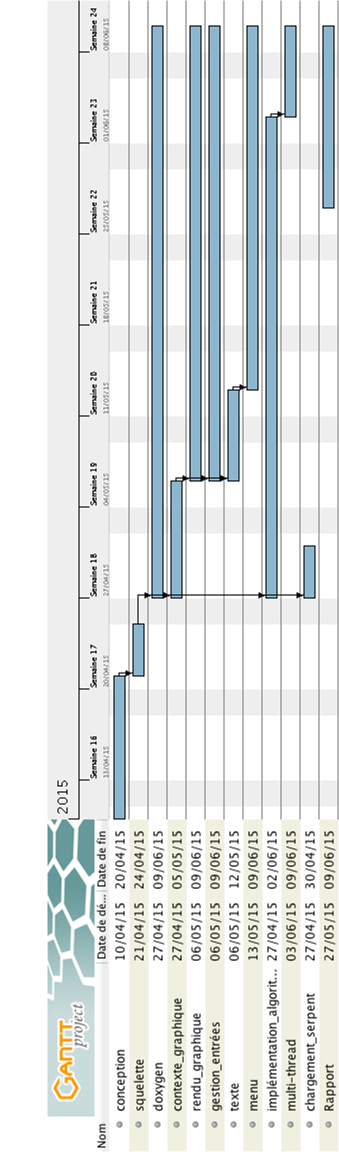
\includegraphics[scale=0.5,keepaspectratio=true]{img/gantt.png}
 \caption{Diagramme de Gantt}
 \label{Gantt}
\end{figure}

\chapter{Architecture logiciel}
Dans ce chapitre, nous allons aborder les aspects techniques liés au développement de notre application.

\section{Le format de fichier ``.snake''}
Les différents snakes proposés par l'application sont stockés dans des fichiers ``*.snake'' dans le répertoire ``Snakes''. Le listing~\ref{.snake} ci-après montre le contenu du fichier ``snake.snake'' soit le serpent chargé par défaut par l'application.\newline

La section \verb|[Volume]| permet de définir les caractéristiques du volume final, soit :
\begin{itemize}
 \item sa largeur (x);
 \item sa hauteur (y);
 \item sa profondeur (z);
 \item l'état de chacun des sous-cubes le formant (x;y;z;State).
\end{itemize}

La première ligne indique les dimensions (maximales, sur les trois axes) du volume final. L'exemple présenté ici indique que le volume à remplir est contenu dans un cube de 3x3x3. 
Ensuite, on associe à chaque triplet de coordonnées un ``état'', matérialisé par la dernière valeur entière de chaque ligne. La valeur 1 signifie que le volume final occupe l'espace à cette coordonnée. La valeur -1 indique au contraire que le volume final ne doit pas occuper cet emplacement.\newline

La section \verb|[Snake]| définit le nombre et l’enchaînement des unités formant le serpent. La valeur 0 indique que l'unité est une extrémité du serpent, la valeur 1 indique une unité de type ``droite'' et la valeur 2 une unité de type ``angle''.\newline

La section \verb|[Symetry]| permet quant à elle de définir quels sont les axes de symétrie à prendre en compte lors de la recherche des vecteurs initiaux (cf partie 3.4). La valeur 1 représente le fait qu'un axe de symétrie est applicable aux faces du volume tandis que la valeur 0 indique qu'il ne convient pas de l'utiliser. Ces quatre entiers correspondent respectivement aux axes de symétrie vertical, horizontal, diagonal anti-slash et diagonal slash.

\newpage
\begin{lstlisting}[caption=Contenu du fichier snake.snake]
 [Volume]
  3;3;3
  0;0;0;1
  0;0;1;1
  0;0;2;1
  0;1;0;1
  0;1;1;1
  0;1;2;1
 
  [ ... ]
 
  2;1;1;1
  2;1;2;1
  2;2;0;1
  2;2;1;1
  2;2;2;1
  [Snake]
  27
  0;1;2;2;2;1;2;2;1;2;2;2;1;2;1;2;2;2;2;1;2;1;2;1;2;1;0;
  [Symetry]
  1;1;1;1
\end{lstlisting}\label{.snake}

\section{L'utilisation des threads}
Nous avons dès le départ pris le parti d'utiliser la technique du multithreading afin de séparer l’exécution du rendu 3D et le reste de l'application. Cela permet notamment de faciliter la gestion des animations et, de manière plus générale, de limiter la dépendance du rendu 3D avec les diverses fonctions de calcul. 

Plus tard dans le développement de l'application, nous avons étendu l'utilisation des threads au calcul des solutions. Cette parallélisation a permit d'améliorer le temps de calcul, en particulier pour le Snake Cube de taille 4x4x4.\newline

Le schéma suivant (Fig.\ref{threads}) montre l'organisation des threads de notre programme. On distingue 4 types de threads :
\begin{itemize}
 \item Le thread principal, qui a pour rôle de créer les autres thread et qui fait donc office de thread de contrôle. C'est également lui qui se charge de l’interaction homme/machine (récupération et interprétation des entrées clavier/sourie).
 \item Le thread graphique à qui il incombe d'actualiser l'écran de sorte à avoir dans l'idéal une fréquence de 60 images par seconde. Ce thread est démarré au lancement du programme et se termine lors de la fermeture du l'application.
 \item Le thread de calcul, dont le rôle est de répartir le travail de recherche des solutions au différents threads de résolution de noeud. Se thread permet de calculer les solutions pour un snake tout en laissant la possibilité à l'utilisateur d'interagir avec l'application (pression sur la touche ``échap'' notamment. Ce thread est démarré en mode détaché pour recherché toutes les solutions lorsque l'utilisateur charge un nouveau serpent. Il peu également être lancé en mode attaché (attente de la fin de l’exécution) lorsque l'utilisateur demande une aide à la résolution. Ce démarrage en mode attaché représente une contrainte que nous n'avons pas eu le temps de contourné. En effet, quand ce thread est en mode attaché, il perd sa capacité à totalement paralléliser le travail de recherche. L'utilisateur ne peut donc plus interagir avec l'application pendant le calcul, le thread principal étant bloqué par l'attente de la fin de l'exécution du thread de calcul.
 \item Les thread de résolution de noeud; ces threads sont créés par le thread de calcul. Il permette d'explorer plusieurs branche de l'arbre de recherche en même temps, permettant ainsi de réduire le temps de calcul. Le nombre de point de départ (de branches) à explorer pour chaque thread de résolution de noeud est définit de la manière suivante : soit n le nombre de thread de résolution de noeud à utiliser et x le nombre de point de départ possible pour résoudre le snake. Le nombre de point départ affectés au n-1 premier thread sera a = x / n. Pour le n\up{ième} thread, le nombre de point de départ affectés sera b = n - ((n-1) * a). Nous verrons dans la partie ``Résultats'' que cette façon de faire présente un inconvénient.
\end{itemize}

\begin{figure}[h]
 \centering
 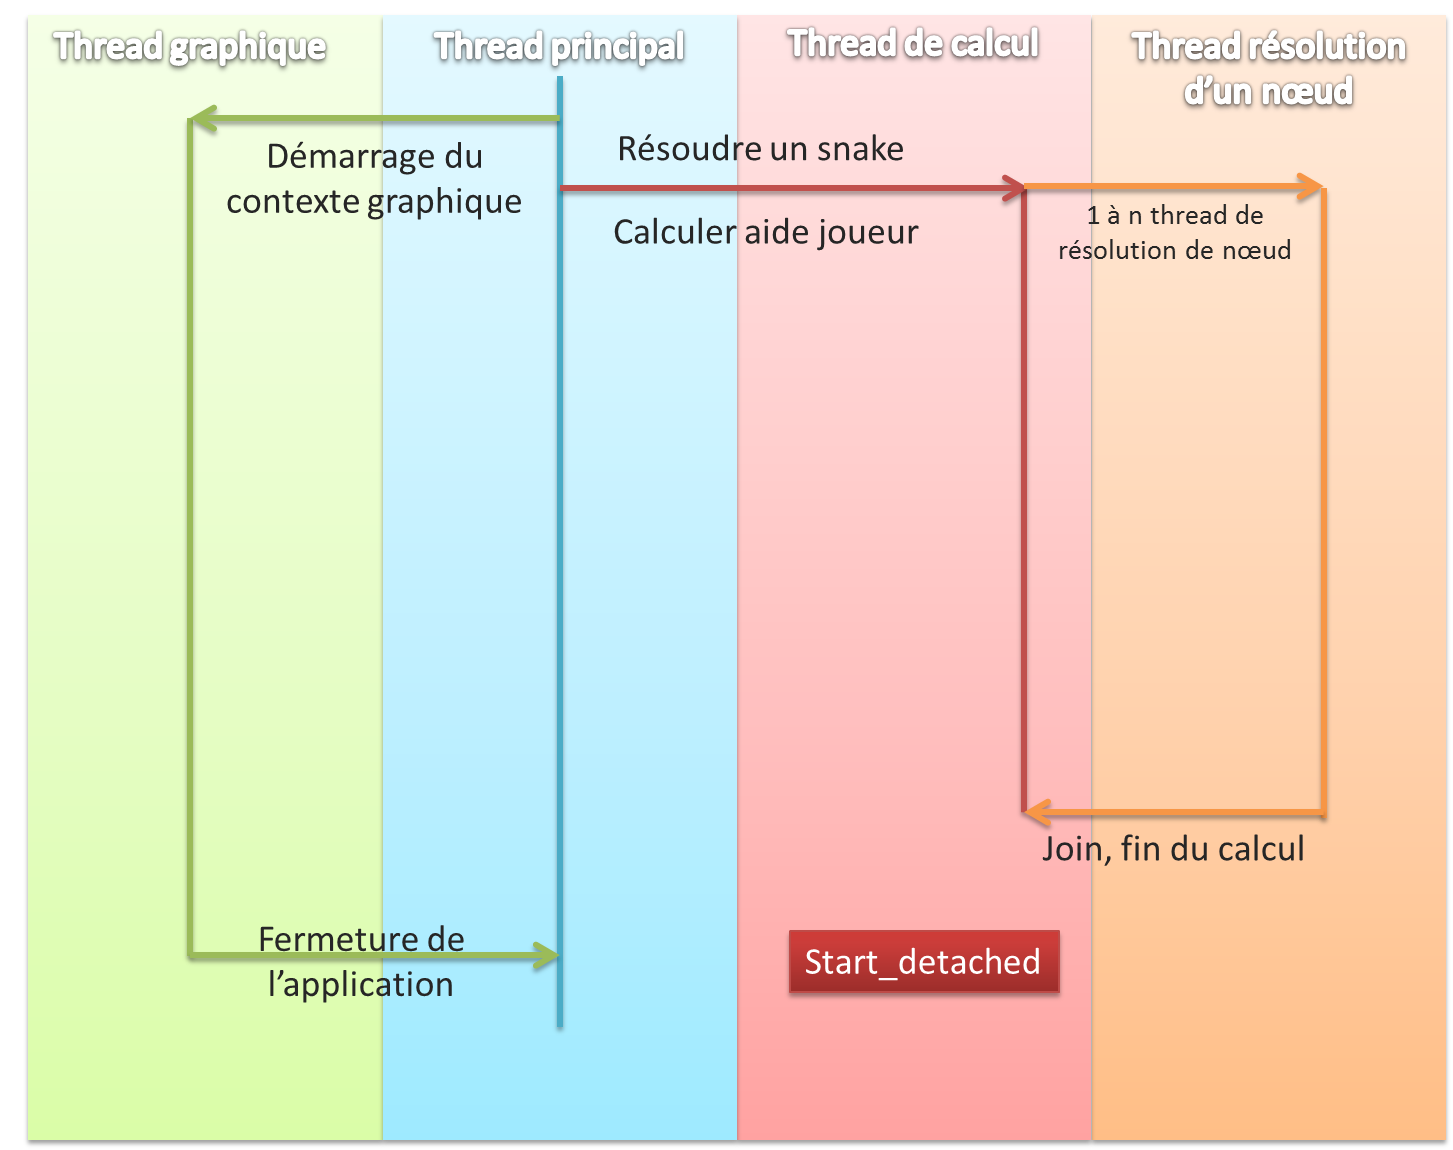
\includegraphics[scale=0.4,keepaspectratio=true]{img/threads.png}
 \caption{Organisation des threads}
 \label{threads}
\end{figure}

\part{Développement}
\chapter{Core}
Il se dégage des objectifs le besoin de présenter à l'utilisateur les solutions du casse-tête et de lui permettre d'interagir intuitivement avec l'application. Afin de répondre à ce besoin, il est nécessaire d'avoir un affichage volumétrique (3d) et une interface permettant la lecture des entrées des périphériques courants (clavier, souris). Nous avons donc décidé d'utiliser OpenGL (Open Graphics Library) comme librairie graphique et GLFW (GL FrameWork) comme librairie de gestion de fenêtre et d'entrées.

Afin de permettre des calculs asynchrones à la représentation graphique du cube serpent, nous avons décidé de créer un thread dédié à cette représentation qui aurait pour but la simple lecture de données relatives au casse tête. En limitant la fréquence de rafraichissement de l'affichage à 60 images/secondes, le temps processeur est épargné de manière à favoriser les calculs relatifs à la résolution,  la fluidité d'affichage est garantie, et les conflits de lecture deviennent très peu fréquents (et même imperceptibles).

\section{OpenGL}

OpenGL (Open Graphics Library) est un ensemble normalisé de fonctions de calcul d'images 2D ou 3D lancé par Silicon Graphics en 1992. Cette interface de programmation est disponible sur de nombreuses plateformes où elle est utilisée pour des applications qui vont du jeu vidéo jusqu'à la CAO en passant par la modélisation.

\begin{quotation}
 OpenGL permet à un programme de déclarer la géométrie d'objets sous forme de points, de vecteurs, de polygones, de bitmaps et de textures. OpenGL effectue ensuite des calculs de projection en vue de déterminer l'image à l'écran, en tenant compte de la distance, de l'orientation, des ombres, de la transparence et du cadrage.\newline
 [source: http://fr.wikipedia.org/wiki/OpenGL]
\end{quotation}

Nous avons choisi de restreindre notre code à la version 2.1 d'OpenGL pour des raisons de compatibilité, celle-ci étant supportée par tous les pilotes de carte graphique récents. Cette version apporte le concept de pipeline programmable: certaines parties de la création d'image sont codées par le développeur, compilées et exécutées par le GPU. Ces programmes sont appelés shaders et permettent un contrôle accru du procédé de calcul d'image.

\begin{figure}[h]
 \centering
 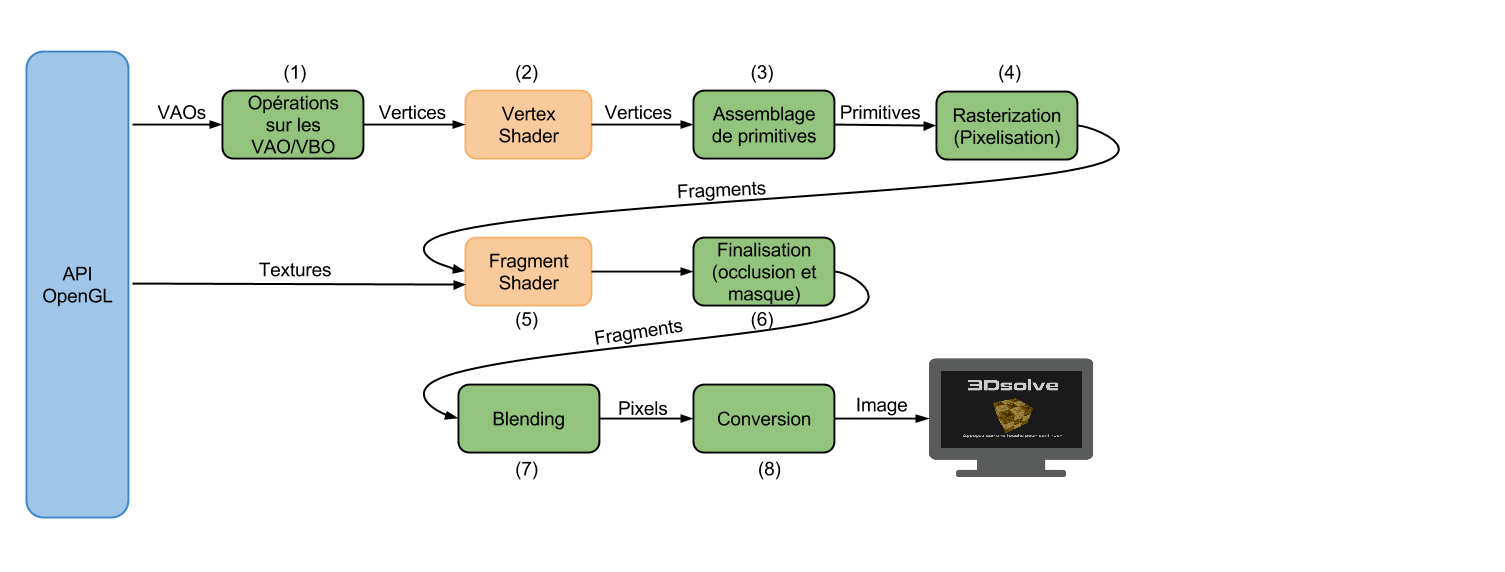
\includegraphics[scale=0.3,keepaspectratio=true]{img/pipeline.png}
 \caption{Le pipeline programmable (simplifié)}
 \label{pipeline}
\end{figure}

Les données (Vertices, UV, textures) et les shaders sont tous chargées dans la mémoire graphique au démarrage du programme, permettant ainsi de réduire grandement le flux de données sur le bus graphique. Ainsi, seuls des identifiants (entiers) sont à communiquer au GPU pour choisir sur quelles données sont exécutées les opérations.
    La figure~\ref{pipeline} détaille les différentes étapes clés du calcul d'une image au sein de la carte graphique:

\begin{enumerate}
 \item Dans le programme, on informe le GPU d'utiliser un VAO (Vertex Array Object), qui va contenir des informations relatives aux vertices (points dans l'espace). Dans notre cas, un VAO contient un tableau de vertices (x, y, z) et un tableau de coordonnées de texture (U, V) pour chaque vertex (ces tableaux sont appelés VBO, Vertex Buffer Object). Cet objet est traité en (1) et execute l'instruction suivante pour chaque vertex du VAO.
 \item Ces vertices sont ensuite traités par le /vertex shader/ (2) (détaillé par la suite), qui effectue des opérations de calcul vectoriel.
 \item Une fois transformés, ces vertices sont assemblés en (3) pour former des primitives. Dans notre cas, une primitive est un triangle, formé par un triplet de vertices adjacents dans le premier tableau du VAO.
 \item Vient ensuite l'étape de rasterization (4): des fragments de pixels sont créés à partir des primitives. Un fragment correspond à une subdivision surfacique de primitive de la taille d'un échantillon de pixel, c'est une conversion d'une information vectorielle vers une information échantillonnée.
 \item Les fragments ainsi créés sont ensuite traités par le /fragment shader/ (5) (détaillé par la suite), qui va "coller" la texture renseignée par le programme sur le fragment en fonction de sa position sur la primitive.
 \item Les fragments ayant les mêmes coordonnées à l'écran sont ensuite ordonnés en fonction de la position de la primitive dont il est issu: un fragment issu d'une primitive cachée par une autre sera placé "derrière" celui issu de la primitive le cachant, quel que soit l'ordre dans lesquels ils ont été traités préalablement (6). Les primitives en arrière plan seront donc partiellement ou totalement occultées.
 \item Ces fragments ordonnées sont ensuite fusionnés en pixels (7). Cette étape réalise deux opérations majoritaires: la fusion de couleur des fragments (en fonction de leur transparence) en échantillons, et le rassemblement de ces échantillons pour former un pixel. L’intérêt de posséder plusieurs échantillons est entre autres l'anti-crénelage (lissage des traits). On peut dire qu'un pixel est issu de n fragments, avec n = nombre d'échantillons * nombre de primitives sous le pixel.
 \item Ces pixels sont ensuite convertis dans le format d'image spécifié par l'application, ici déterminé par le système d'exploitation, puis affichés à l'écran.
\end{enumerate}

\section{Données}
Les données contenues dans les VAO et les textures sont issues de fichiers afin de faciliter leur création et leur modification. On peut trouver les modèles 3D dans le dossier "stc" et les textures dans le dossier "textures".

Nous avons adopté deux formats de modèles 3D différents au cours du développement, STC (format propre) et le format OBJ de WaveFront (très courant grâce à sa simplicité de codage). Le format STC décrit les données telles qu'elles seront agencées dans les VAOs tandis que le format OBJ est plus complexe, mais globalement plus pratique. Il contient une suite de vertices (préfixe "v"), de vecteurs normaux (préfixe "vn"), de coordonnées de texture (préfixe "vt") et des descripteurs de primitives (préfixe "f") associant pour chaque primitive trois triplets (vertex/normale/coordonnée de texture). Une fois décodé, ces données sont transférées dans la mémoire graphique par les VAOs.

Pour les textures, nous avons choisi d'utiliser le format PNG, pour sa compression sans perte, son canal de transparence et son format largement documenté. La bibliothèque lodePNG a été utilisée pour décoder ces textures de manière simple. Une fois décodées, elles sont transférées dans la mémoire graphique par des "texture buffers".

\section{Utilisation des données}
Les vertices des VAO ne contiennent que des coordonnées relatives au centre de l'objet, il est donc nécessaire de les transformer dans l'espace afin de les déplacer, de les faire tourner et de changer leur échelle. Ces opérations sont réalisées au travers de calcul matriciel à l'intérieur du /vertex shader/. En effet, les GPU sont optimisés afin de réaliser de nombreuses multiplication matricielles à la chaîne. Voici une partie du code de notre vertex shader principal:\newline

\verb|gl_Position = VP * W * vec4 (vertex_position, 1.0);|\newline

Dans ce code on renseigne au GPU la nouvelle position de notre vertex, multiplié par deux matrices. La première, VP (View-Projection) correspond à la matrice de projection de l'espace en trois dimensions vers un espace en deux dimensions (Calculée à partir de la caméra) et la deuxième, W (World position) correspond à la position de l'objet dont est issu le vertex dans cet espace en trois dimension.

Ces matrices ne sont modifiés qu'une fois par image (alors que tous les vertices sont calculés à chaque image), il est donc judicieux de les calculer par le CPU et de les envoyer via le bus graphique. La matrice VP est calculée en fonction de la caméra, qui est modifiée par les actions de l'utilisateur. La matrice W est calculée par rapport à la position d'un cube dans notre espace en trois dimension virtuel.

Le fragment shader quant à lui permet de "coller" une partie de texture préalablement choisie sur un fragment. Cette opération est effectuée grâce aux coordonnées de texture (UV): elles permettent de relier un vertex (x, y, z) à un point d'une texture (u, v), ce qui permet de déformer la texture en déformant la primitive associée.

\begin{figure}[h]
 \centering
 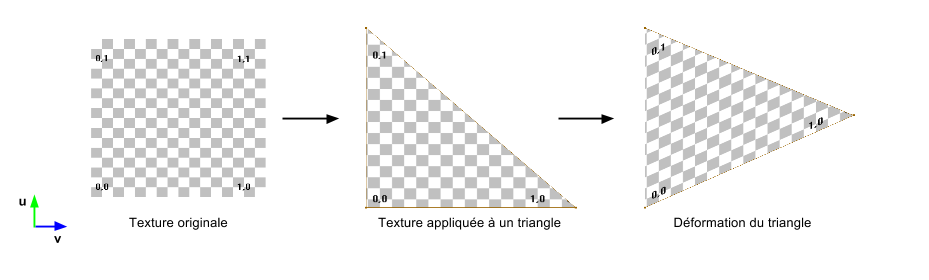
\includegraphics[scale=0.4,keepaspectratio=true]{img/uvexpl.png}
 \caption{Explication UV}
 \label{uv}
\end{figure}

Voici une partie du code de notre fragment shader principal:\newline

\verb|gl_FragColor = vec4(texture2D( CurTex, UV ).rgb, alpha);|\newline

Dans ce code, on renseigne au GPU d'aller chercher une portion de texture à la coordonnée (u, v), de lui ajouter une valeur de transparence arbitraire définie dans notre programme et de l'associer au fragment traité.
\chapter{Graphique}
Toujours dans l’objectif de fournir une application la plus simple a utiliser nous avons décider de dédier une partie du développement au support des différentes plateformes. Bien que compliquée, notre application peut être compilé et exécutée sur les 3 principaux systèmes d’exploitation du marché à savoir :

\begin{itemize}
 \item GNU Linux
 \item Microsoft Windows
 \item OSX Apple
\end{itemize}

Pour la compilation, diverses bibliothèques nécessitent d’être installées (voir le README fournis avec les sources). Le Makefile détecte l’OS utilisé et adapte la chaine de compilation pour la plateforme adéquate. Nous avons également utilisé les commandes préprocesseur de détection de système d’exploitation afin d’avoir un fichier source commun aux différentes plateformes de compilation.

Par ailleurs l’application peut être lancée sur des machines n’ayant pas ces bibliothèques installées grâce à la compilation statique. Les résultats sont encourageants, sur une vingtaine de machines testées seules quelques une ont échouées au lancement du programme. L’application est donc prête a un déploiement et une distribution multi-plateforme.

La compatibilité graphique a été un vrai défi puisque nous avons travaillé avec certains types de données d’OpenGL 3 au début du projet, il s’est avéré malheureusement que certaines de nos machines nécessaires aux tests de portabilités n’acceptaient que des fonctions jusqu’à OpenGL 2.1 et certaines extensions. 

Le développement et l’adaptation des techniques de rendu a donc été adapté pour répondre a ces contraintes de versions.
\chapter{Portabilité}
\section{Résolution d'un Snake Cube}
L'objectif visant à résoudre un Snake Cube est atteins. Notre application propose divers Snake Cube et les résout en un temps raisonnable (voir Chapitre~\ref{Tests}). En plus de résoudre des Snake Cube classique, c'est à dire dont la forme finale est un cube, notre application peut également résoudre des Snake dont la forme finale est plus complexe. Nous avons par exemple créer un Snake dont la forme finale peut être apparenté à un temple maya (\verb|snake_maya_temple.snake|).

\begin{figure}[h]
 \centering
 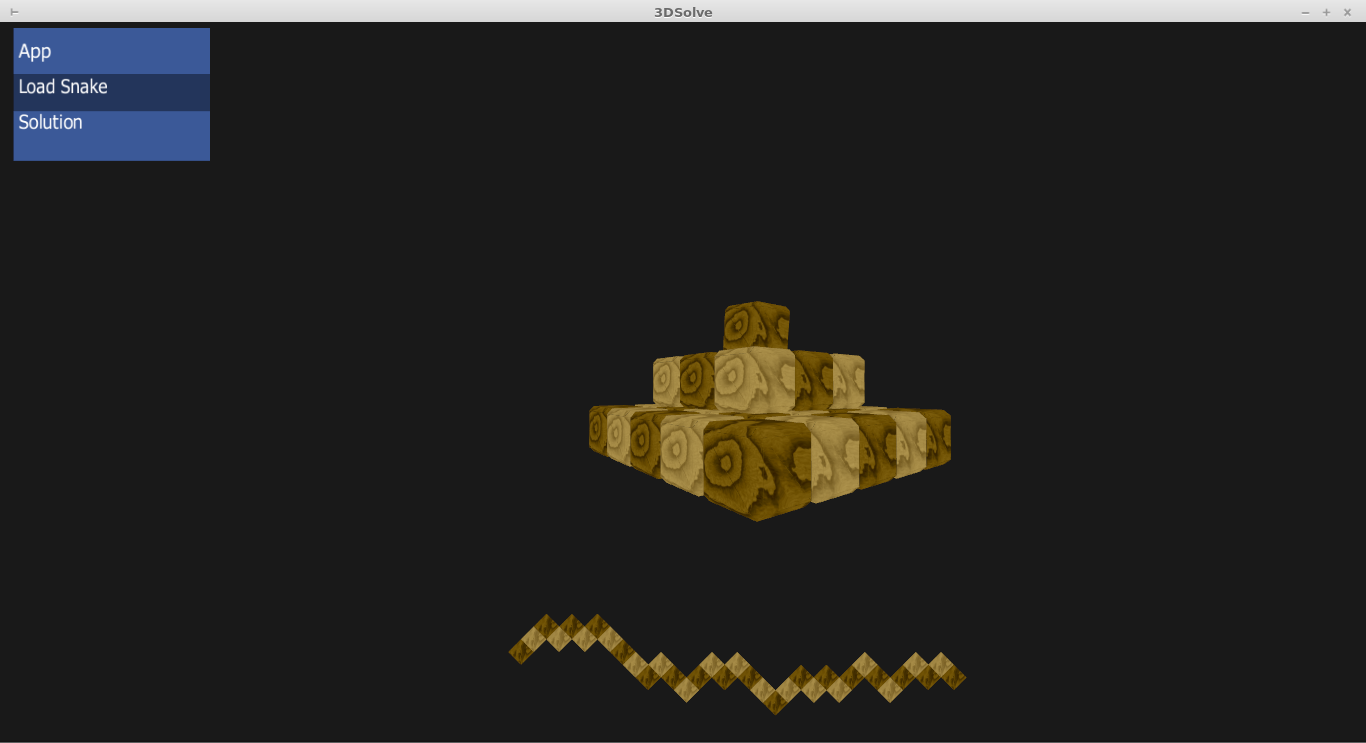
\includegraphics[scale=0.3,keepaspectratio=true]{img/screenShot3.png}
 \caption{``Temple maya'' résolu}
 \label{screenShot3}
\end{figure}

L'interface de rendu 3D propose à l'utilisateur de visualiser, à son rythme, les diverses solutions menant à la résolution du casse-tête sélectionné.

\newpage
\section{Interactivité avec l'utilisateur}
L'objectif d'interactivité avec l'utilisateur, autrement dit la possibilité donné à l'utilisateur de résoudre lui-même le casse-tête, est également atteint. En effet, notre application propose une interface 3D permettant à l'utilisateur de manipuler virtuellement le casse-tête et finalement, un pris d'un effort cérébrale non-négligeable, de le résoudre.

\begin{figure}[h]
 \centering
 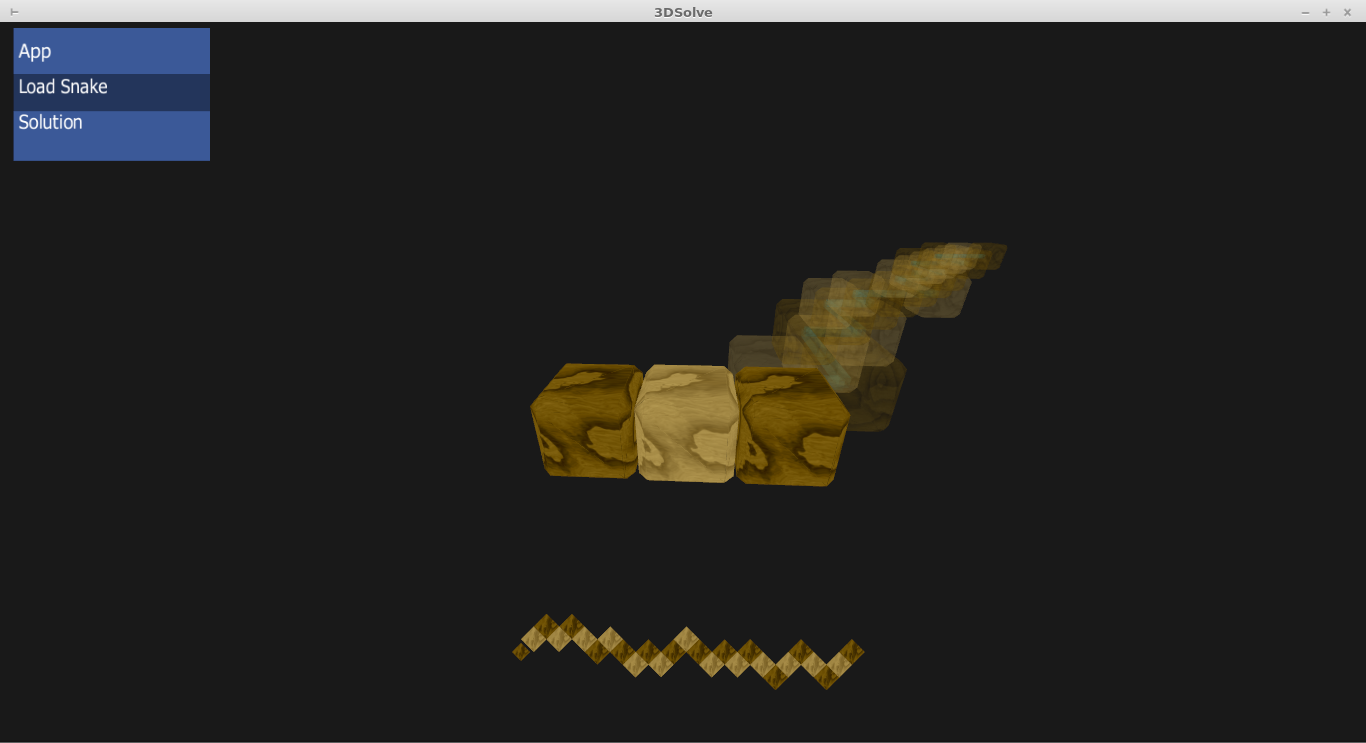
\includegraphics[scale=0.3,keepaspectratio=true]{img/screenShot1.png}
 \caption{Snake Cube déplié en attente de résolution}
 \label{screenShot1}
\end{figure}

\section{Amélioration proposée}
Nous avons eu diverses idées que nous aurions aimé implémenté si nous avions eu plus de temps. Nous les avons regroupées ici sous une seul et même proposition d'amélioration.

L'amélioration consiste en un éditeur de snake. Cet éditeur, sous la forme d'une interface dans le contexte de rendu 3D, permettrait à l'utilisateur de créer ses propres casse-tête.

En premier lieu, l'éditeur pourrait proposer à l'utilisateur de définir un volume en 3D puis de passer ce volume à un algorithme qui effectuerait le travail inverse de l'algorithme de résolution. C'est-à-dire qu'à partir du volume qui lui est donné, il créer un ou plusieurs enchaînement d'unité de snake et créé donc un casse-tête. Le snake ainsi créé pourrait ensuite être sauvegardé dans le format définit au chapitre~\ref{ch6} et être ensuite utilisé comme les autres snake dans la partie interactive de l'application.

Ensuite, on pourrait également imaginer que cet éditeur permette à l'utilisateur de définir non seulement un volume mais également l'enchaînement des unités du snake afin de modéliser un snake réel qui n'est pas proposé par l'application.


\part{Résultat}
\chapter{Réalisations}
\section{Test n°1}

\begin{description}
 \item[Date]: 18/05/15
 \item[Sur code révisé]: commit f7da39f0001d221ccd82f236781b4c97f7f9ca88
 \item[OS]: Linux Mint 17 Cinnamon 64-bit
 \item[Noyau Linux]: 3.31.0-24-generic
 \item[Processeur]: Intel© Core™ i5-3230M CPU @ 2.60GHz * 2
 \item[Type d'algorithme]: mono-thread
 \item[Objectif]: Prouver l'utilité de l'algorithme de réduction des points de départ.
\end{description}

\begin{table}[h]
\begin{tabular}{|*{5}{c|}}
\hline
Algorithme&Taille du cube&Temps de calcul (s)&Solutions&Chemins explorés \\
\hline
\multirow{3}{*}{Actif}&2x2x2&0,000429&6&38 \\
&3x3x3&0,047914&32&91 347 \\
&4x4x4&140,208572&11&615 765 110 \\
\hline
\multirow{3}{*}{Inactif}&2x2x2&0,005929&144&889 \\
&3x3x3&0,781355&576&1 922 269 \\
&4x4x4&2985,381852&192&11 258 895 649 \\
\hline
\end{tabular}
\caption{Résultats du test n°1}
\end{table}

\newpage

\paragraph{Interprétation} La première interprétation que l'on peut faire de ces résultats est que, sans surprise, plus la taille du cube est grande, plus le temps de calcul est important (0,000429 secondes pour un 2x2x2 contre 140,208572 pour un 4x4x4). Ces résultats nous permettent également de prouver l'efficacité de notre algorithme de réduction des points de départ. En effet, lorsque l'algorithme est actif on constate que les temps de calcul, tout comme le nombre de chemins explorés, sont plus faibles que lorsque qu'il est inactif.

\begin{figure}[h]
 \centering
 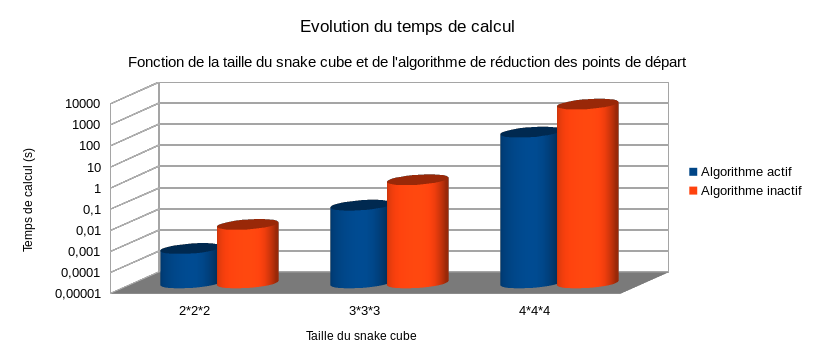
\includegraphics[scale=0.6,keepaspectratio=true]{img/test1.png}
 \caption{Graphique test n°1}
\end{figure}

\newpage

\section{Test n°2}

\begin{description}
 \item[Date]: 30/05/15
 \item[Sur code révisé]: commit c8d1b7bdf5eb1f94255cd66aca9b0b800cba838d
 \item[OS]: Linux Mint 17 Cinnamon 64-bit
 \item[Noyau Linux]: 3.31.0-24-generic
 \item[Processeur]: Intel© Core™ i5-3230M CPU @ 2.60GHz * 2
 \item[Type d'algorithme]: mono-thread ou multi-thread
 \item[Objectif]: Évaluer l'efficacité de la parallélisation du calcul des solutions.
\end{description}

\begin{table}[h]
\begin{center}
\begin{tabular}{|*{2}{c|}}
\hline
\multicolumn{2}{|c|}{Snake 3x3x3} \\
\hline
Nombre de thread & Temps d’exécution (s) \\
\hline
1 & 0,002462 \\
\hline
2 & 0,001642 \\
\hline
3 & 0,003461 \\
\hline
4 & 0,002232 \\
\hline
5 & 0,002773 \\
\hline
6 & 0,002652 \\
\hline
7 & 0,002292 \\
\hline
8 & 0,001988 \\
\hline
9 & 0,002477 \\
\hline
10 & 0,002387 \\
\hline
\end{tabular}
\end{center}
\caption{Résultats du test n°2-1}
\end{table}

\begin{table}[h]
\begin{center}
\begin{tabular}{|*{2}{c|}}
\hline
\multicolumn{2}{|c|}{Snake 4x4x4} \\
\hline
Nombre de thread & Temps d’exécution (s) \\
\hline
1 & 99,067031 \\
\hline
2 & 67,078735 \\
\hline
3 & 65,022525 \\
\hline
4 & 53,198234 \\
\hline
5 & 47,776286 \\
\hline
6 & 71,80401 \\
\hline
7 & 54,967149 \\
\hline
8 & 47,836183 \\
\hline
9 & 45,215047 \\
\hline
10 & 45,38195 \\
\hline
\end{tabular}
\end{center}
\caption{Résultats du test n°2-2}
\end{table}

\newpage

\paragraph{Interprétation} Le temps de résolution du snake 3x3x3 étant très court, l'efficacité du calcul parallèle est difficile à percevoir. De plus, l'influence d'autres processus s'exécutant sur la même machine que l'application biaise certainement les résultats pour ce snake. Le cas du snake 4x4x4 est plus intéressant. On constate que plus on affecte de threads à la résolution du calcul, moins celui-ci prend de temps. Ceci se vérifie jusqu'au 5e thread. Ensuite, on observe un ``pic'' dans le temps de calcul, puis il décroit de nouveau. Selon nous, ce pic est dû à la façon dont nous avons implémenté le système de répartition des points de départ à traiter pour chaque thread. Dans ce cas précis, il y a 10 points de départ à traiter. Si l'on utilise 6 threads de calcul, le programme affecte (10 / 6) = 1 point de départ pour chaque thread, excepté le dernier auquel il affecte (10 - 5) = 5 threads. Finalement, avec ce système, on constate que la parallélisation du calcul n'est vraiment pas optimale, ce qui explique le ``pic '' dans le graphe.

\begin{figure}[h]
 \centering
 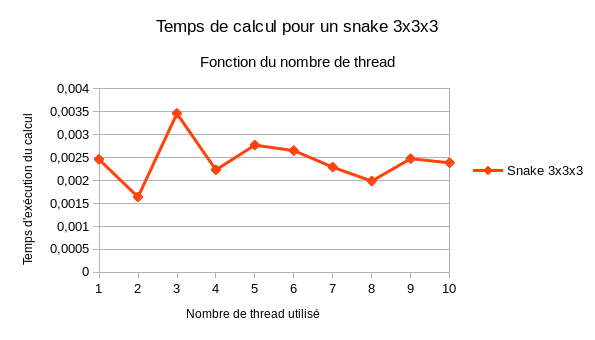
\includegraphics[scale=0.7,keepaspectratio=true]{img/test2-1.png}
 \caption{Graphique test n°2-1}
\end{figure}

\begin{figure}[h]
 \centering
 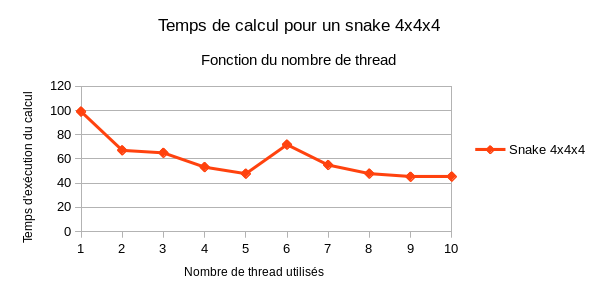
\includegraphics[scale=0.7,keepaspectratio=true]{img/test2-2.png}
 \caption{Graphique test n°2-2}
\end{figure}

\section{Limites}
Nos tests nous ont permis de mettre en évidence la limite principale de notre application : la taille du cube à résoudre. En effet, pour un cube 4x4x4 le temps d'attente n'est déjà plus négligeable et sa résolution sollicite grandement le CPU. 
\chapter{Tests}
Dans le but de vérifier l'efficacité de certains de nos algorithmes, de connaître les performances ainsi que les limites de notre application, nous avons effectué plusieurs benckmark donc voici les résultats et conclusions.

\textbf{Benckmark n°1}


\listoffigures
\lstlistoflistings

\printindex
\end{document}